%This is a Latex file.
\documentclass[12pt]{article}
\usepackage{latexsym,fancyhdr,amsmath,amsfonts,amsthm,dsfont}
\usepackage{amssymb}
\usepackage{tikz}
\usetikzlibrary{graphs}
\usepackage{graphicx} 

% margins are relative to the default of 1 in
%\topmargin       -0.2 in

\topmargin        -0.2 in
\textheight       8.4 in
\oddsidemargin    0 in     % this is for pages 1, 3, 5, ...
\evensidemargin   0 in     % and this for 2, 4, 6, ...
\textwidth        6.5 in
%\headheight       15 in     % we won't have a running head, nor
\headsep          .35 in     % any extra space between head and text

%\parindent 0pt

\pagestyle{fancy} \lhead{\sf MTH 317} \chead{\sf Homework \#?}
\rhead{\sf Your Name} \lfoot{} \cfoot{} \rfoot{}

\newcommand{\C}{\mathds{C}}
\newcommand{\I}{\mathds{I}}
\newcommand{\N}{\mathds{N}}
\newcommand{\Q}{\mathds{Q}}
\newcommand{\R}{\mathds{R}}
\newcommand{\Z}{\mathds{Z}}
\begin{document}
\begin{enumerate}
\item[2.20]  Show that if G is a connected graph that is not regular, then G contains adjacent vertices
 u and v such that deg(u) $>$ deg(v).

    
\item[2.22] 
\begin{center}
    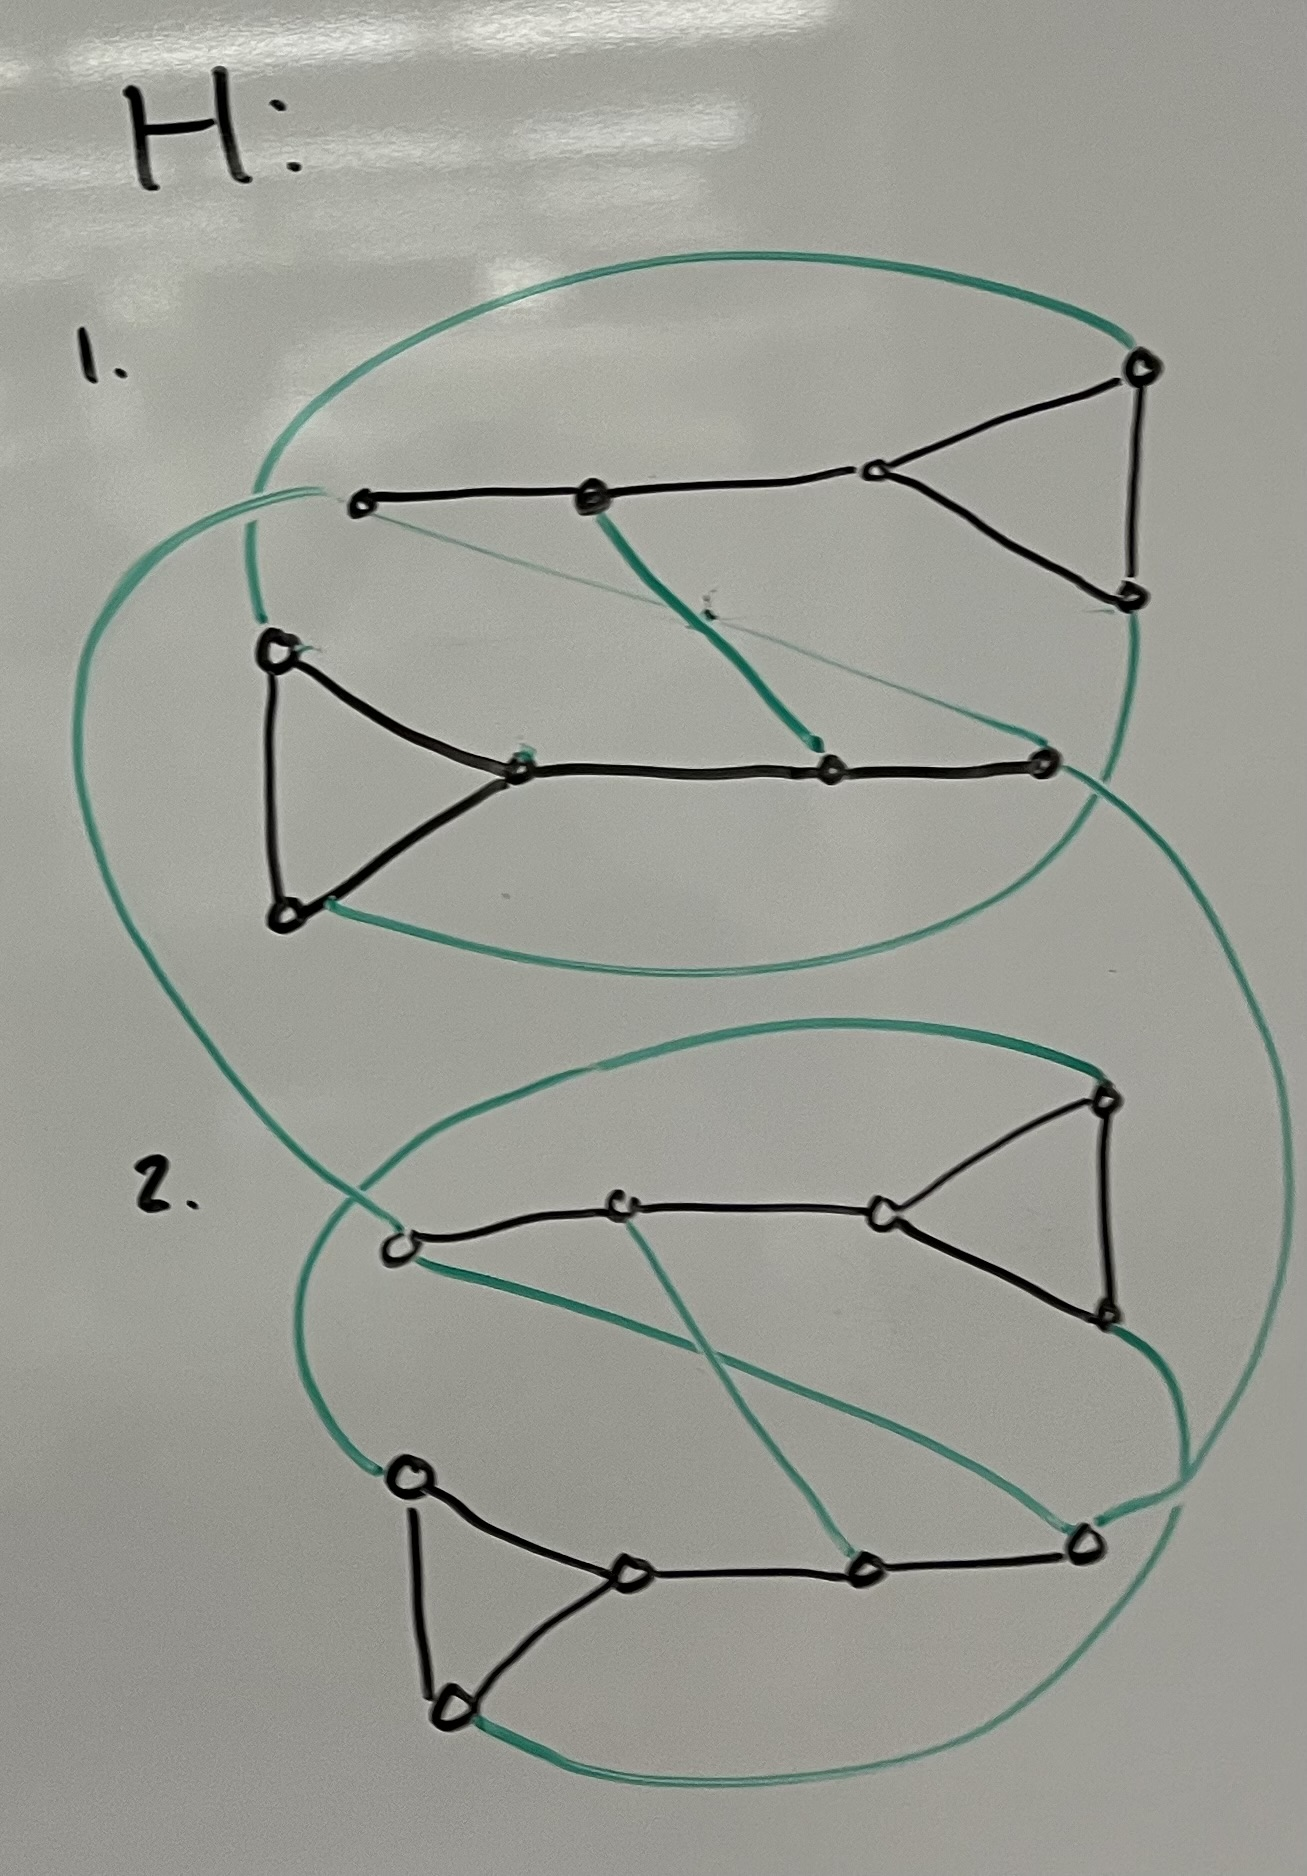
\includegraphics[width=0.5\textwidth]{IMG_1782.jpg}
    order = 20
\end{center}

\item[2.26]
\item[2.32] Determine if the following sequences are graphic. If so, construct a graph.
\item[b] 

    Start: 6,3,3,3,3,2,2,2,2,1,1
    \newline
    Remove 6 and subtract 1 from the first 6 remaining numbers: 2,2,2,2,1,1,1,1,1,1
    \newline
    Remove 2 and subtract 1 from the first 2 remaining numbers: 1,1,2,1,1,1,1,1,1
    \newline
    Remove 2 and subtract 1 from the first 2 remaining numbers: 1,1,1,1,1,1,1
    \newline
    Remove 1 and subtract 1 from the first remaining number: 1,1,1,1,0
    \newline
    Remove 1 and subtract 1 from the first remaining number: 1,1,0,0,0
    \newline        
    Remove 1 and subtract 1 from the first remaining number: 0,0,0,0
    \newline
    All zeros, so the sequence is graphic.


\item[d] 
\begin{center}
    Start: 7,5,4,4,4,3,2,1
    \newline
    Remove 7 and subtract 1 from the first 7 remaining numbers: 4,3,3,3,2,1,0
    \newline        
    Remove 4 and subtract 1 from the first 4 remaining numbers: 2,2,2,1,0,0
    \newline
    Remove 2 and subtract 1 from the first 2 remaining numbers: 1,1,1,0,0,0
    \newline        
    Remove 1 and subtract 1 from the first remaining number: 1,1,0,0,0
    \newline
    Remove 1 and subtract 1 from the first remaining number: 1,0,0,0,0
    \newline        
    Remove 1 and subtract 1 from the first remaining number: 0,0,0,0
    \newline
    All zeros, so the sequence is graphic.

\end{center}
\item[2.33]


\end{enumerate}
\end{document}
